\textbf{\LARGE{Part one: Design Project}}

This report suggests a strategy for improving the booking system
of \gomonkey{}, taking into account the current state of the company both as a
business and as a company with a pre-existing organizational
structure that endorses certain work practices and processes to support
sustaining and growing the company.

\section{Knowledge required to understand the design project}
This report is the result of a comprehensive case study following the \must{ } method. 
\must{ } rests on the principles of a multi-phase analysis that
culminates in one or more \textit{visions} for success that take the current
situation of the company into account. Such a vision can be used by \gomonkey{}
to initiate or discard the changes suggested, doing so on the basis of an
\textbf{informed choice}. The report further serves as a blueprint for
\textit{how} to transition to a future organization incorporating the needed
changes, on an organizational as well as technical level.

Much effort has been devoted to understanding the \textbf{reasons} for why the
current work practice exists, indeed this concept is a core part of an
ethnographically inspired design project. This kind of analysis has qualities
that are often attributed with IT project success, see for example The Standish
Group's CHAOS summaries that discuss key factors in IT project success and
failure.

The report is split into two primary sections: one that describes the current
work practices, environment and organization, and another that proposes change
based on the existing situation and aims to reach goals and solve specific
problems identified.

\subsection{Focus area and motivation}
Very early on, \gomonkey{} and the design team came to an agreement about the
focus of the project: the on-line booking system. The system is regarded as
complex and undocumented by both the design team and the manager of \gomonkey{}, 
Michel Pascual. This leads to issues in passing on responsibility. One of the
first things said about this were:

\begin{quotation}
I don't dare let my employees handle the bookings!

\em - Michel Pascual, manager and owner of \gomonkey{}, 15.10.2013
\end{quotation}

There is fear that employees will make a mistake in the process given the
complexity and lack of documentation of the booking system. Add to this the many
different ways bookings are handled and the large amount of manual communication
needed and it quickly becomes apparent that the booking process is not only
difficult but currently almost undefined. At the same time, bookings take a
considerable amount of time to process, and as \gomonkey{} is a newly started
company there are perhaps other things that Michel might be able to spend his
time on to better grow the company, if it was possible.

\section{Business strategy}
No formal business strategy was available from \gomonkey{}, possibly owing to
the fact that the company is so new. The design team constructed a lightweight
business strategy, essentially equivalent to a list of goals.

\begin{enumerate}
	\item Become a self-sustainable climbing company with customers on a daily basis.
	\item Minimize time requirements pr.\ booking/customer.
	\item Minimize staff requirements to keep costs low.
	\item Increase sales (such as selling food and drinks).
	\item Provide better and more comprehensive services than competitors.
    \item Continue to run the main site on WordPress, to preserve an SEO
        advantage.
\end{enumerate}

The purpose of this prioritized list of business goals is to relate decisions
made and solutions proposed directly or indirectly to a specific point in the
business strategy, to help ensure that the solution is focused on furthering
actual business goals and creating value for the company.

\section{Work domains}
The core business of \gomonkey{} is to sell climbing sessions. However, there
are a number of auxiliary work processes as well which may or may not be profit-related
but mandatory all the same. 

The identified work domains are listed in \autoref{table:workdomain}.

\begin{table}[H]
    \centering
\begin{tabular}{|l|l|}
        \hline
        Work domain & Example work processes \\ \hline
        \multirow{4}{*}{Booking Flow} 
            & Registering received bookings \\
            & Checking payment status \\
            & Informing customers prior to arrival \\
            & Receiving customers \\
        \hline
        \multirow{3}{*}{Employee Schedule} 
            & Scheduling shifts \\
            & Swapping shifts \\
            & Time registration \\
        \hline
        \multirow{2}{*}{Economy and bookkeeping} 
            & Payment during booking \\
            & Invoice after visit \\
        \hline
        \multirow{2}{*}{Inventory Management} 
            & Maintenance of inventory \\
            & Stock control of equipment \\
        \hline
        \multirow{2}{*}{Marketing} 
            & Advertising \\
            & Offers and discounts \\
        \hline
\end{tabular}
\caption{List of work domains and example work processes in specific work domains}
\label{table:workdomain}
\end{table}

The obvious work domain that overlaps with the focus of the design project is
that of the booking flow. While the other work domains are important aspects of
\gomonkey{}, no time will be spent fleshing out those work domains unless it is
relevant to the primary focus of the booking system, or considered an achievable
``nice to have''.

\subsection{Existing work practices and problems}
After analysing work practices at \gomonkey, we consider the following situations 
critical in improving the booking process. Although these situations can be taken
in sequential order, they were analysed individually.

\begin{description}
\item[Initial Booking]
A potential customer which has landed on the website can initiate a booking
by clicking "Book Tid" to access the booking form. He then has to fill in his name, e-mail, phone number, 
the desired booking date and time, the number of persons that will be joining and their
age span along with any additional notes he might have. 
After the user has filled in the form, he is taken to a confirmation
page and two e-mails are sent: one to the manager with the booking information from the form and
one to the customer informing them that \gomonkey{} has received their booking request. The process
can be followed in \autoref{fig:customer}.

\begin{figure}[htbp]
    \centering
        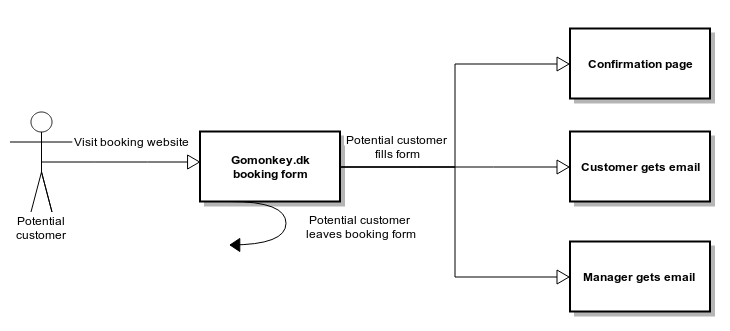
\includegraphics[width=\textwidth]{figures/customer.png}
            \caption{Overview of an initial booking.}
        \label{fig:customer}
\end{figure}

\item[Processing a booking] The manager checks his e-mail for a new booking
    request. If the booking request has any missing information, he contacts the
    customer.  He and the customer communicate over e-mail until all missing
    information is supplied.  An overview of this can be seen in
    \autoref{fig:manager}.  After the customer has supplied all the requested
    information, the manager then enters the information in Google Calendar,
    linking the e-mail with the event. A confirmation e-mail is sent to the
    customer to inform him the booking is scheduled.  Gathering of additional
    booking information through e-mail is done manually and is tedious. This can
    simply be avoided by building a more complex booking system. 

\begin{figure}[htbp]
    \centering
        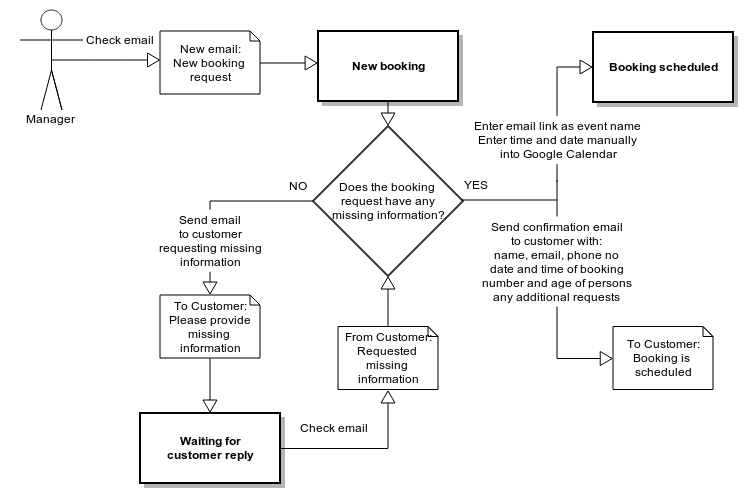
\includegraphics[width=\textwidth]{figures/manager.png}
            \caption{Overview of a booking processing.}
        \label{fig:manager}
\end{figure}

\item[Processing payment]
As seen in \autoref{fig:payment}, the manager is also the one who is processing payments. Every two days
he visits his netbank's website, enters his creditentials then logs into his netbank account. He clicks 
"Recent transactions" and proceeds to  associate recent transactions with their respective bookings in Google Calendar. 
Sometimes customers forget to write their name on their transaction and that leaves the manager unable to identify the customer. 
Having to do everything manually leaves room for human error, a situation which should be avoided. Finally, the manager colors the event associated with the booking
in Google Calendar(blue for fully paid and green for partially paid) and also changes its description to reflect payment status.

\begin{figure}[htbp]
    \centering
        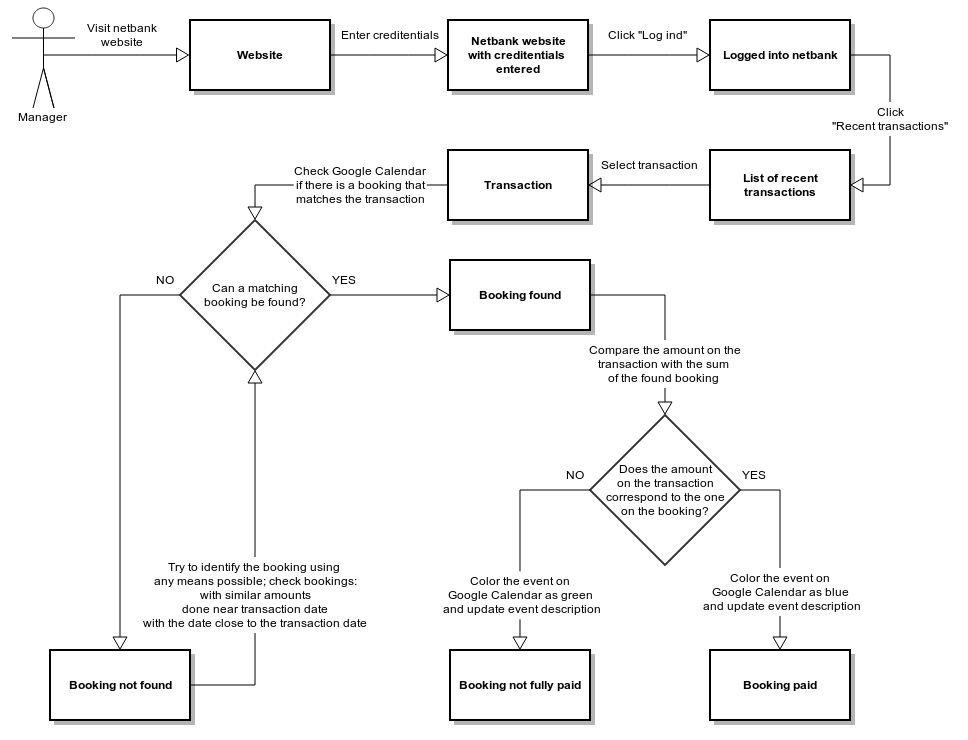
\includegraphics[width=\textwidth]{figures/payment.png}
            \caption{Overview of payment processing.}
        \label{fig:payment}
\end{figure}

\item[Handling booked customers] On the booked time and date, the customer
    arrives at \gomonkey{}. If he has not printed and signed the security
    disclaimer at home, he is handed out one for each member of the group. After
    taking care of the legal requirements, the instructor present proceeds to
    calculate the remaining sum to be paid by the customer, if any. He uses a
    calculator to add up what the customer has left to pay from the booking and
    any extra services the customer might want. If the sum which to be paid is
    non-zero the customer is asked whether he wants to pay by creditcard or
    cash. Based on the customer's preferences, the instructor requests payment
    accordingly. After the customer has paid or if the sum on the calculator is
    0 the handling procedure is over.  The instructor can either be the employee
    present that day at \gomonkey{} headquarters or the manager. The process is
    shown in \autoref{fig:handling}. 

\begin{figure}[htbp]
    \centering
        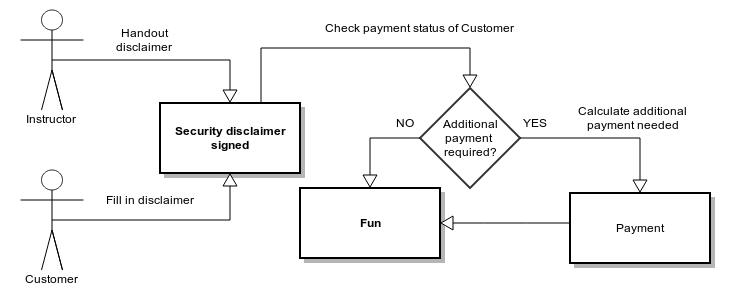
\includegraphics[width=\textwidth]{figures/handling.png}
            \caption{Overview of customer handling}
        \label{fig:handling}
\end{figure}
\end{description}

\section{Identified problems with current work practice}
A number of different techniques were employed by the design team to arrive at a
list of potential problems that warrant fixing. Employees of \gomonkey{} were
interviewed and observed, potential customers were observed while conducting
bookings and the work practices and organization of \gomonkey{} were sketched out
and analyzed. This led to a list of problems, the top five of which are
presented here as items that are considered to be of \textbf{high} importance
for \gomonkey{} to solve, based on the goals of the company and this project.

\begin{itemize}
	\item Customer is disgruntled by the interface.
    \begin{itemize}
        \item Confirmed through observing a potential customer making a booking.
    \end{itemize}
	\item Required complex e-mail communication with customer concerning routine questions
        \begin{itemize}
            \item Confirmed by examining past e-mail communication between
                \gomonkey{} and customers, as well as interviews with the
                Manager of \gomonkey{}.
        \end{itemize}
	\item Payment is cumbersome and slow and error-prone.
        \begin{itemize}
            \item Confirmed by examining the potential error possibilities that
                can occur in relation to a payment.
        \end{itemize}
	\item Entering a booking into the system is cumbersome.
        \begin{itemize}
            \item Confirmed by interviewing the Manager of \gomonkey{} and
                analysis of video material during an observation of this task.
        \end{itemize}
	\item Calculating deficit payment amount at arrival of a booked group is
        troublesome.
        \begin{itemize}
            \item Described in an interview with Nanna, as a potentially
                troublesome task.
        \end{itemize}
\end{itemize}

\newpage
\section{A coherent vision for change}
In the following section we will describe how the technical and
organizational aspects of \gomonkey{} can transition to a point where the
problems identified previously are solved. Such a solution requires not only
changes to the IT infrastructure of \gomonkey{}, but also potentially to the way
day-to-day work is conducted. This occurs naturally because a new IT system
can introduce changes that permeate throughout the entire company structure.

The proposed solution is to contract the building of a custom software for
booking, which can then be hosted on a server that \gomonkey{} will
control. The solution fits within the requirements of the business and adheres
to the business goals, in particular it also respects the requirement to keep
the main site within \texttt{WordPress}.

The booking system is described in the following section through a series of
described mockups. Following the system description are estimates for cost,
proposed organizational changes, required customer and employee qualifications
and an implementation strategy which details how to realize the vision. Lastly,
we briefly discuss an alternative to a custom system at the end.

\subsection{Components, functions and interface of the booking system}
The new booking system contains 5 components, described by a mockup image that
focuses on the functionality of the component. Each mockup has an associated
description that explains how the component works. Lastly, we discuss how the
new components solve the initial problems that were considered high priority.

The mocked up components are
\begin{itemize}
    \item A customer booking process
    \item A customer payment process
    \item An administrative overview of bookings
    \item An administrative processing of a new booking
    \item An administrative overview of the current days bookings
\end{itemize}

\autoref{fig:bookinitial} supports `A customer booking process', incorporating
many of the original features and functions of the existing booking form. New
fields have been added to support an expanded amount of cases, such as ordering
food. The user must input values into the booking form. A price calculator is
available on the right-hand side of the booking form, providing a running total
of the cost of the booking as well as any deposit, if the booking warrants one.
In addition, a Frequently Asked Questions section has been located directly in
the booking form, to prevent navigation-related issues from trying to find
answers to common questions in menus and submenus of the website.

\begin{figure}[htbp]
    \centering
        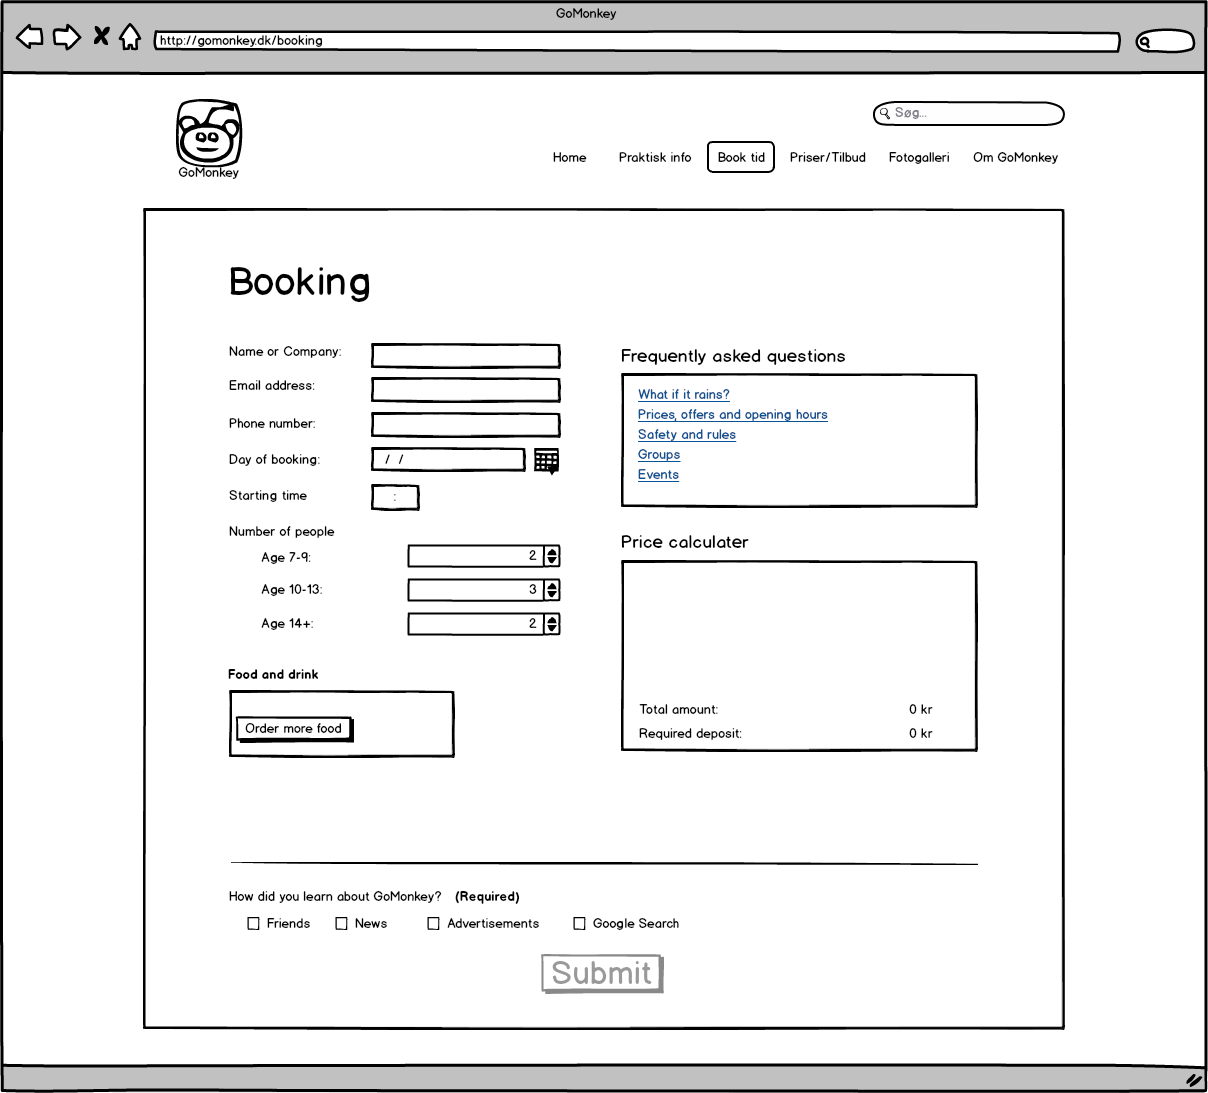
\includegraphics[width=.6\textwidth]{figures/mockup/booking_initial.png}
	    \caption{The bare booking form which the customers will find on the WordPress website.}
        \label{fig:bookinitial}
\end{figure}

An example of a filled booking page can be seen in \autoref{fig:bookfilled}.
The system will ensure that all data is entered in a valid way, such that the
form will not allow an invalid booking. This could be a booking with zero
participants, or a date that has already passed. The \textbf{Submit} button will
transfer the user to a confirmation page described below.

\begin{figure}[htbp]
    \centering
        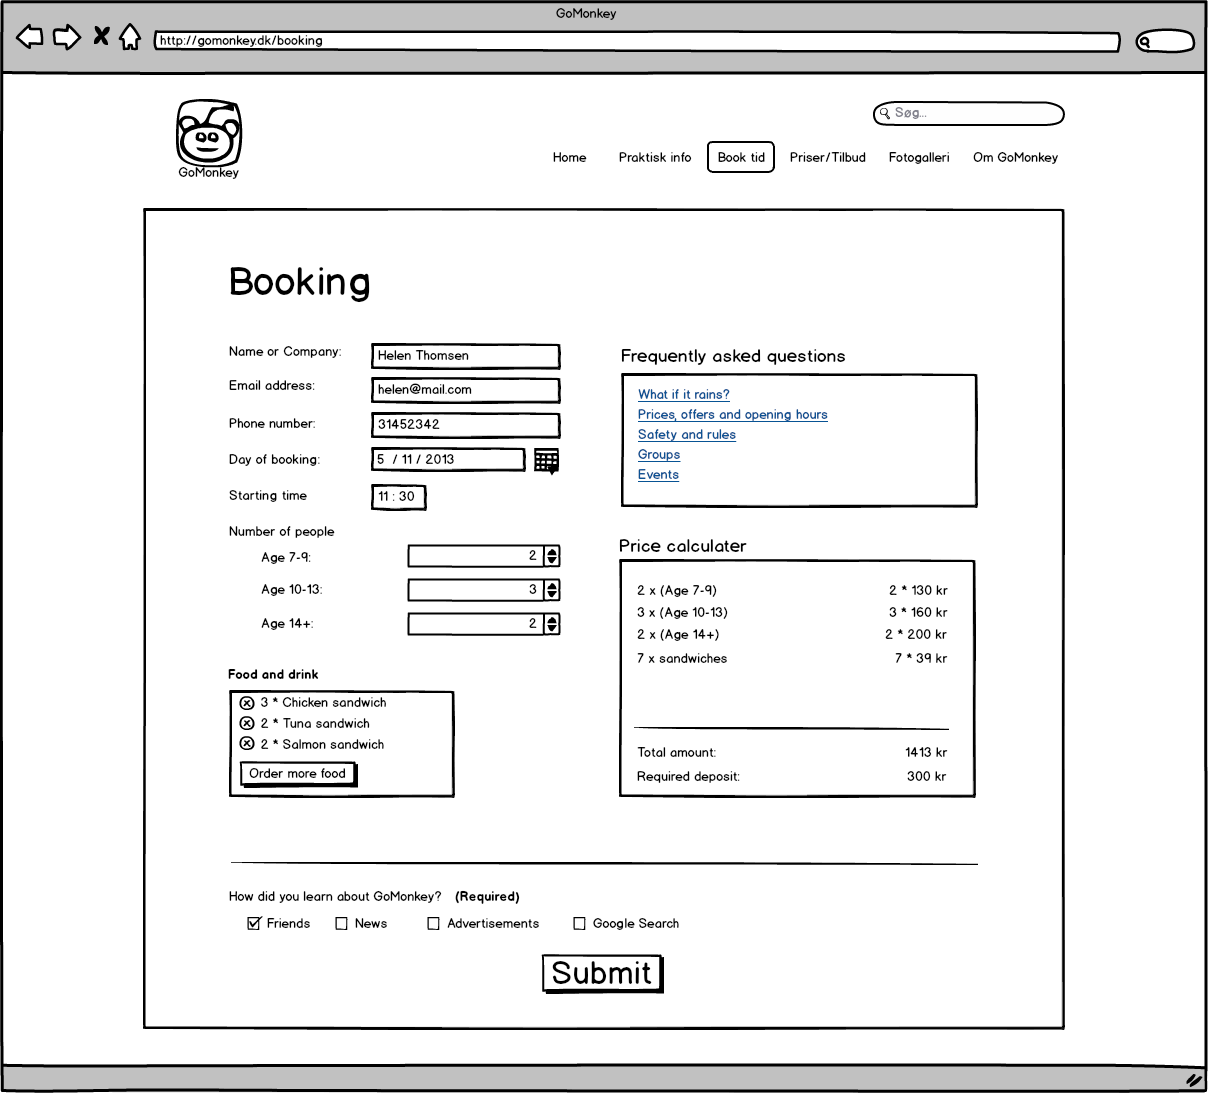
\includegraphics[width=.6\textwidth]{figures/mockup/booking_filled.png}
	    \caption{The booking form is filled and ready to be submitted.}
        \label{fig:bookfilled}
\end{figure}

The confirmation page seen on \autoref{fig:bookconfirm} is reached by clicking
the \textbf{Submit} button from the booking form. If the data entered is
incorrect, the user may go back to editing the booking by clicking the
\textbf{Back} button.

\begin{figure}[htbp]
    \centering
        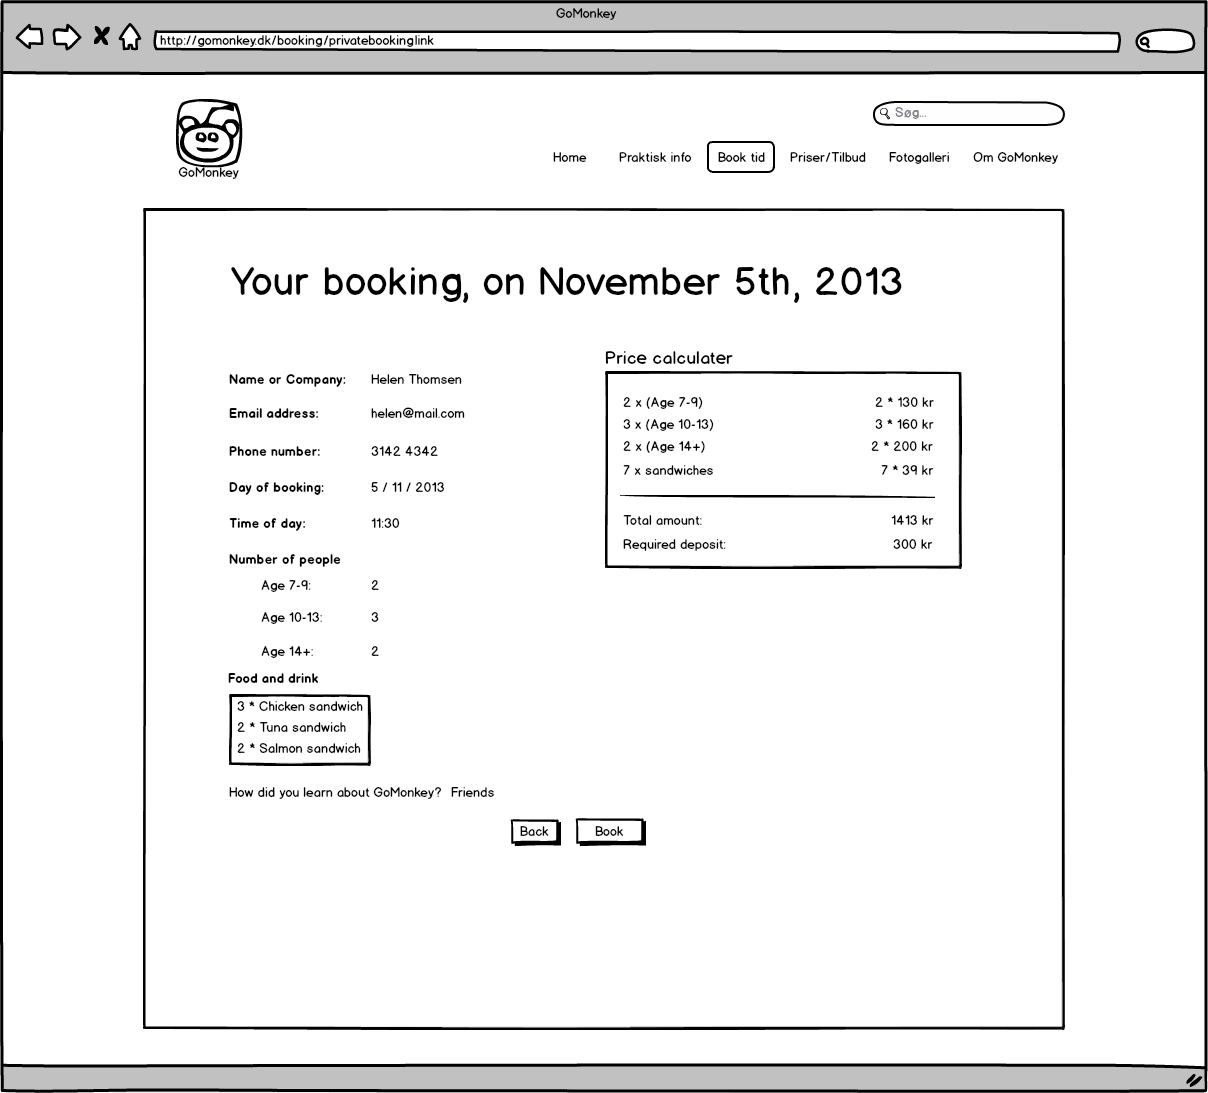
\includegraphics[width=.6\textwidth]{figures/mockup/booking_confirmation.png}
	    \caption{The booking form is submitted and the customer can view the entered information before finally booking.}
        \label{fig:bookconfirm}
\end{figure}

If the user agrees to the entered information, the
user can click \textbf{Book} and the booking will be sent while the user is presented
with a modal popup that informs them that the booking will need to be confirmed,
and that there might be a required deposit. This can be seen on \autoref{fig:bookconfirmpressed}.
Closing the modal popup sends the user on to the booking payment page seen in
\autoref{fig:bookstatus1}, and also prompts the system to provide the user with
a link to this page.

\begin{figure}[htbp]
    \centering
        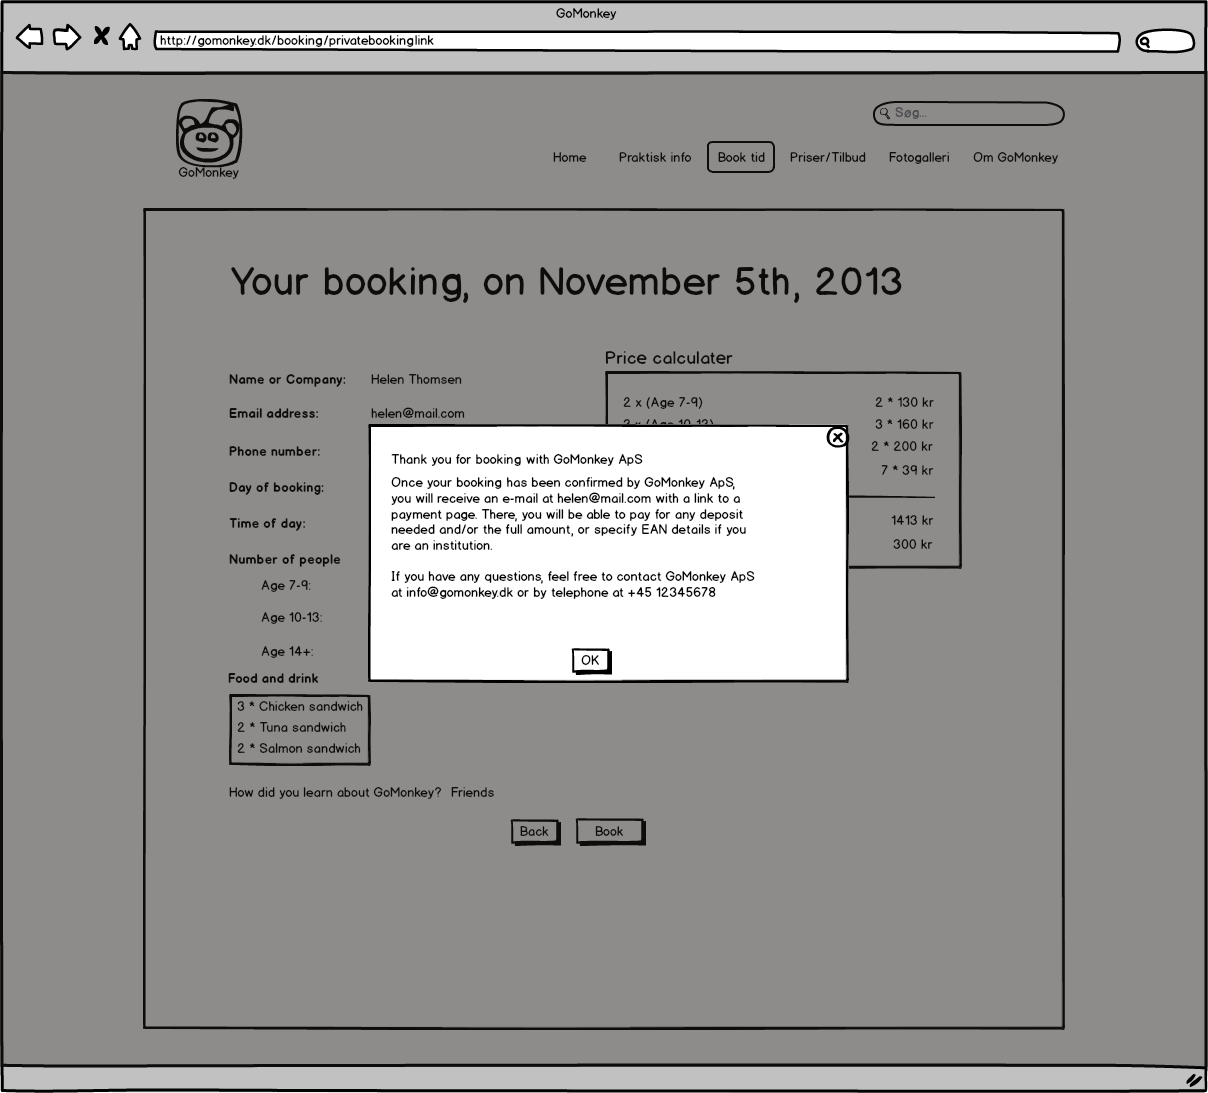
\includegraphics[width=.6\textwidth]{figures/mockup/booking_confirmation_bookpressed.png}
	    \caption{The booking form is submitted and the customer is informed about the following process.}
        \label{fig:bookconfirmpressed}
\end{figure}

\FloatBarrier
\newpage

Unconfirmed bookings cannot yet be paid for in any way. This prevents
\gomonkey{} from having to transfer funds back for a booking that gets declined
after a customer would potentially pay for it. Once a booking is confirmed by
\gomonkey{}, the payment options appear for the customer and an e-mail is sent
to the customer with a link to the customer payment page.

The page supporting `A customer payment process' looks quite similar to the
booking form, but the user cannot make any changes to the booking. In addition
to a list of all the things the user could see in the booking form, the user can
also see whether \gomonkey{} has confirmed the booking or not. An unconfirmed
booking can be seen in \autoref{fig:bookstatus1}, a confirmed booking in
\autoref{fig:bookstatus2}.

\begin{figure}[htbp]
    \centering
        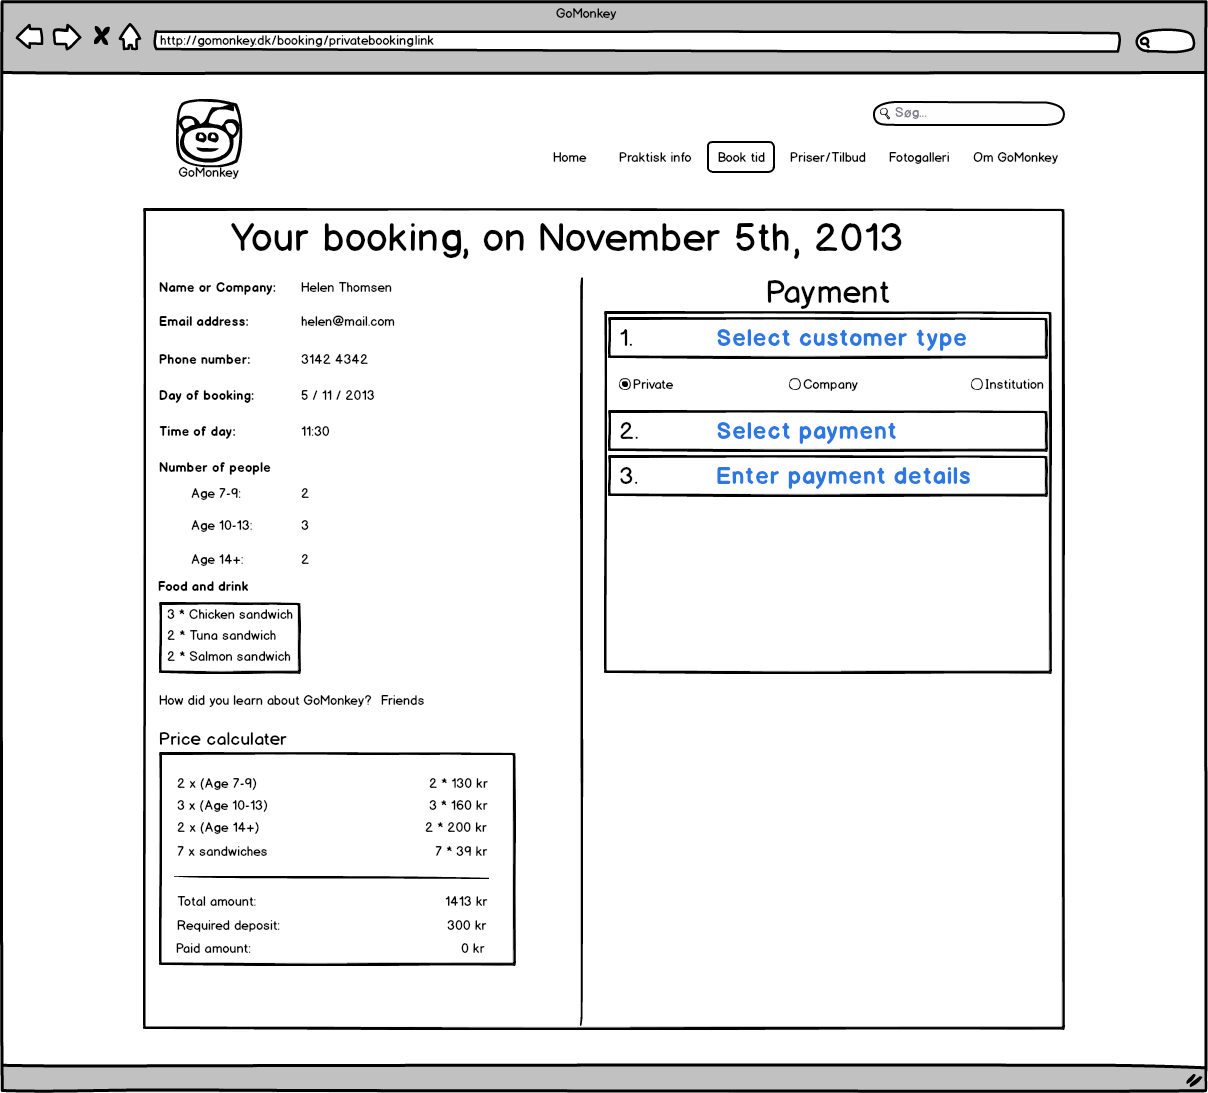
\includegraphics[width=.6\textwidth]{figures/mockup/booking_payment_1.png}
	    \caption{The customer can see the booking, but can't pay until the date and time has been confirmed.}
        \label{fig:bookstatus1}
\end{figure}

The kind of payment must be selected, either a payment for the amount of the
deposit or a payment for the total amount of the booking. Once this has been
selected, options related to a payment processor appear.


\begin{figure}[htbp]
    \centering
        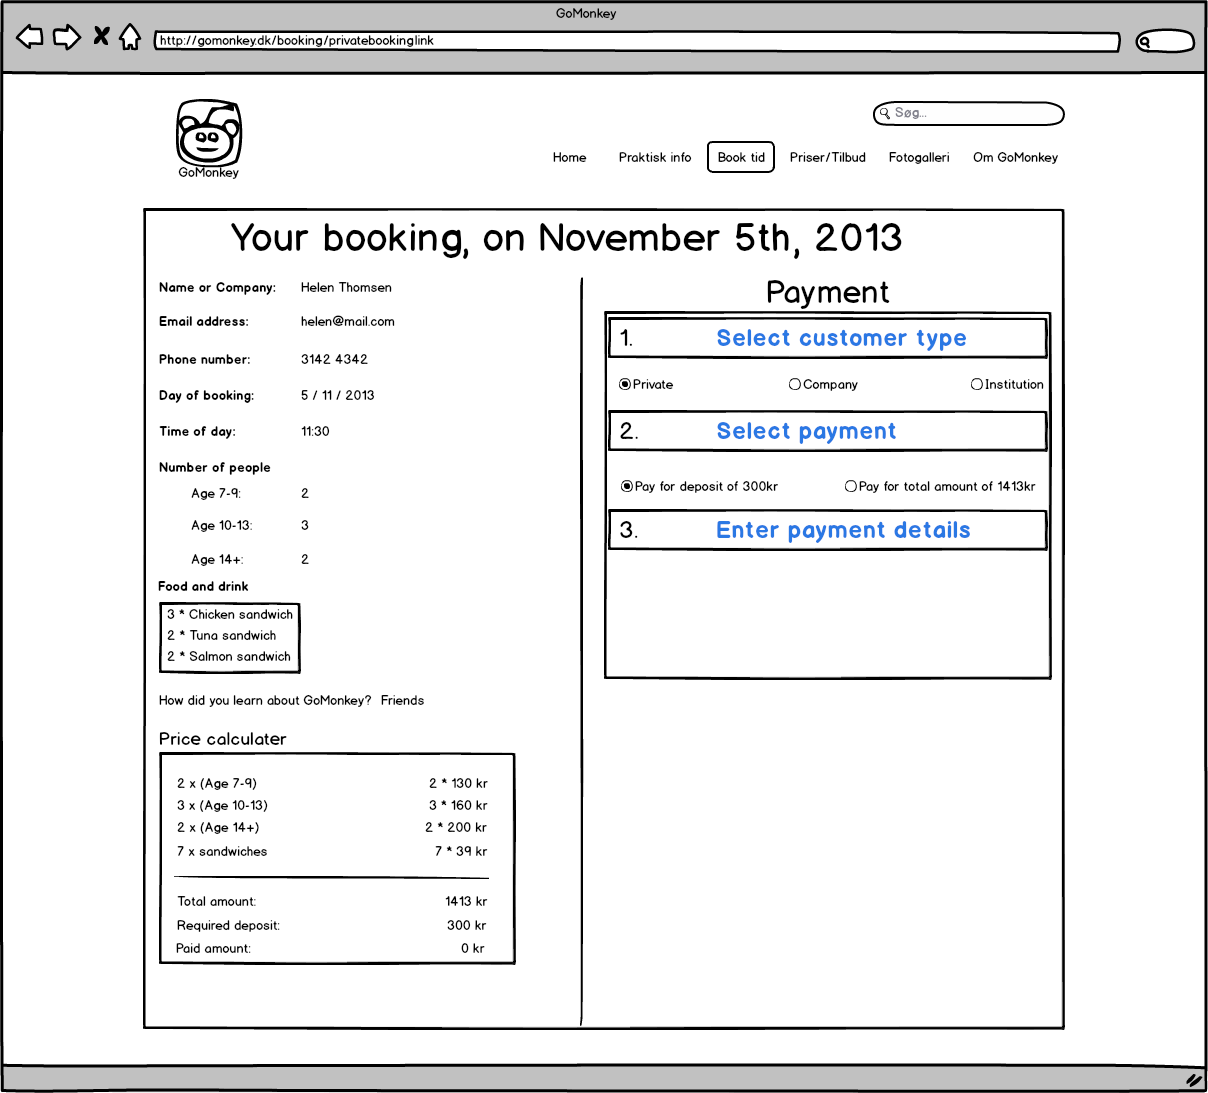
\includegraphics[width=.6\textwidth]{figures/mockup/booking_payment_2.png}
	    \caption{The customer is now able to select the desired amount to be paid, prior to visiting the park.}
        \label{fig:bookstatus2}
\end{figure}

For companies and private persons, payment occurs by clicking on the `Pay via
\ldots' buttons. For public institutions, fields to enter \textit{EAN}-related
details appear. \gomonkey{} will then manually bill the institution using these
details. \autoref{fig:bookstatus3} shows a mockup of payment options for a
private person.

\begin{figure}[htbp]
    \centering
        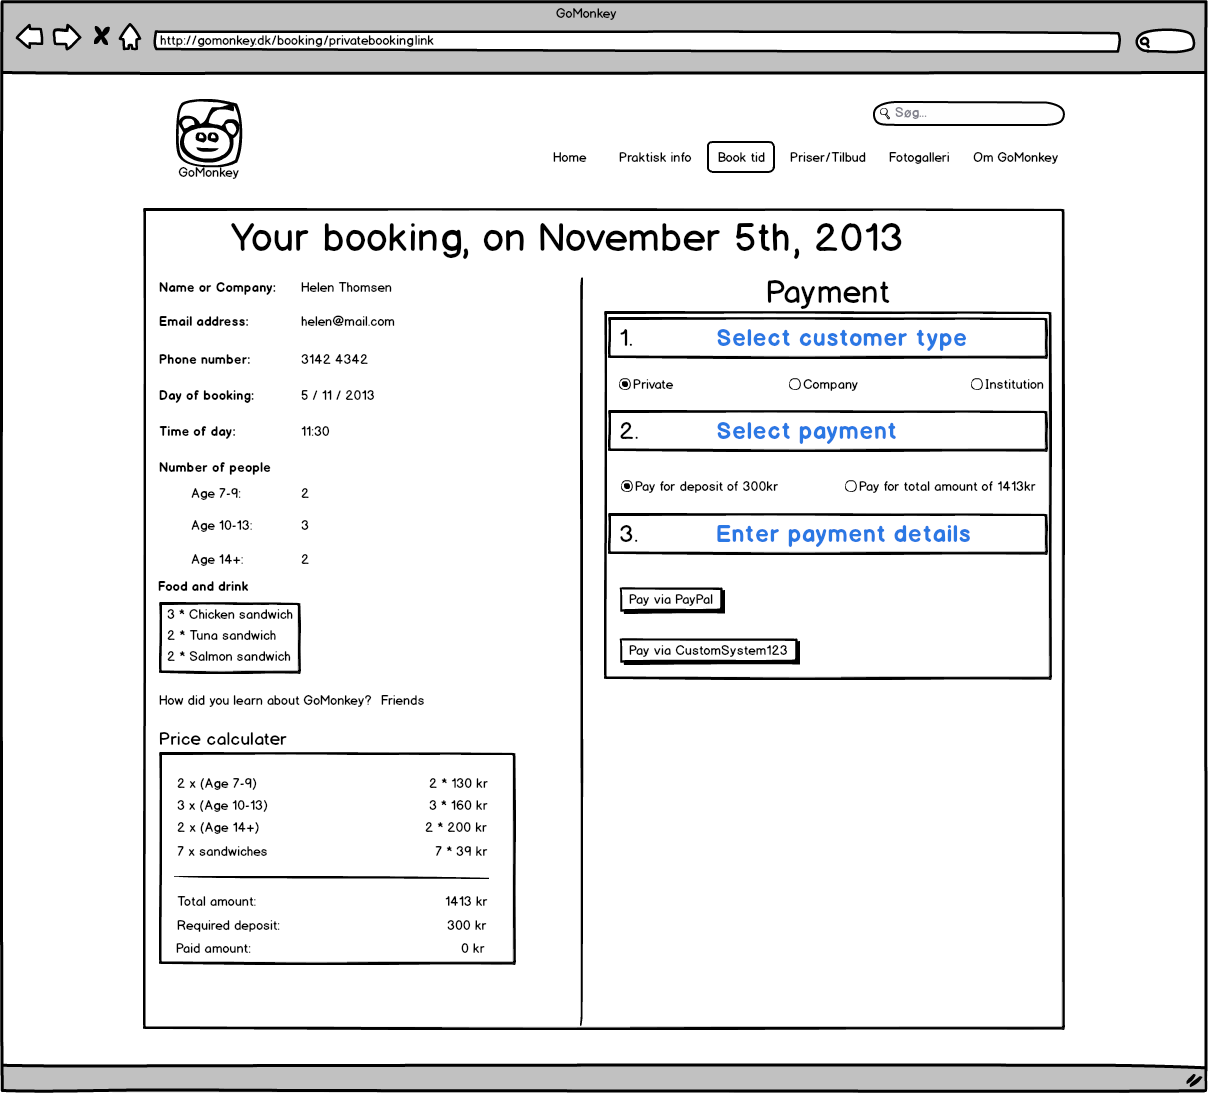
\includegraphics[width=.6\textwidth]{figures/mockup/booking_payment_3.png}
	    \caption{Finally, the customer can select a preferred payment processor and pay instantly.}
        \label{fig:bookstatus3}
\end{figure}

\FloatBarrier
\newpage


The page supporting `An administrative overview of bookings' displays a list of
bookings that require action by the administrator, as seen in
\autoref{fig:adminoverview}. The date, time and amount of people in the 3 age
groups are shown for a quick overview. 

\begin{figure}[htbp]
    \centering
        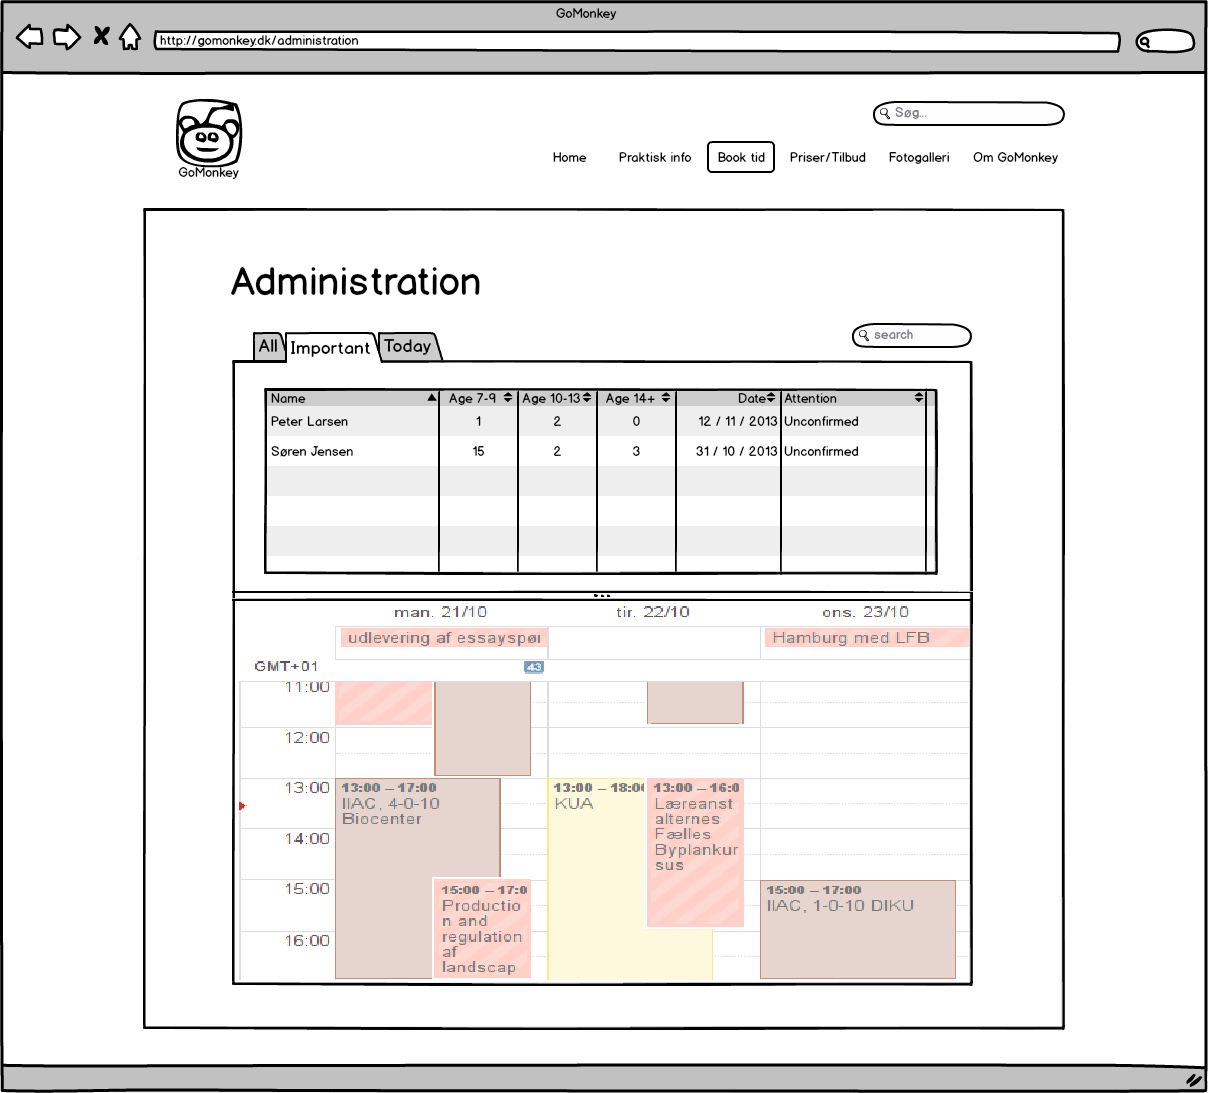
\includegraphics[width=.6\textwidth]{figures/mockup/overview_important.png}
	    \caption{The manager has a good overview of the incoming bookings which requires a reaction.}
        \label{fig:adminoverview}
\end{figure}

\FloatBarrier
\newpage

The page supporting `An administrative processing of a new booking' shows the
entered data for a single booking. This page allows the administrator to either
confirm a booking or decline it. A calendar overview is provided for easy
overview of the day of the booking and surrounding dates, as seen in
\autoref{fig:admin}.

\begin{figure}[htbp]
    \centering
        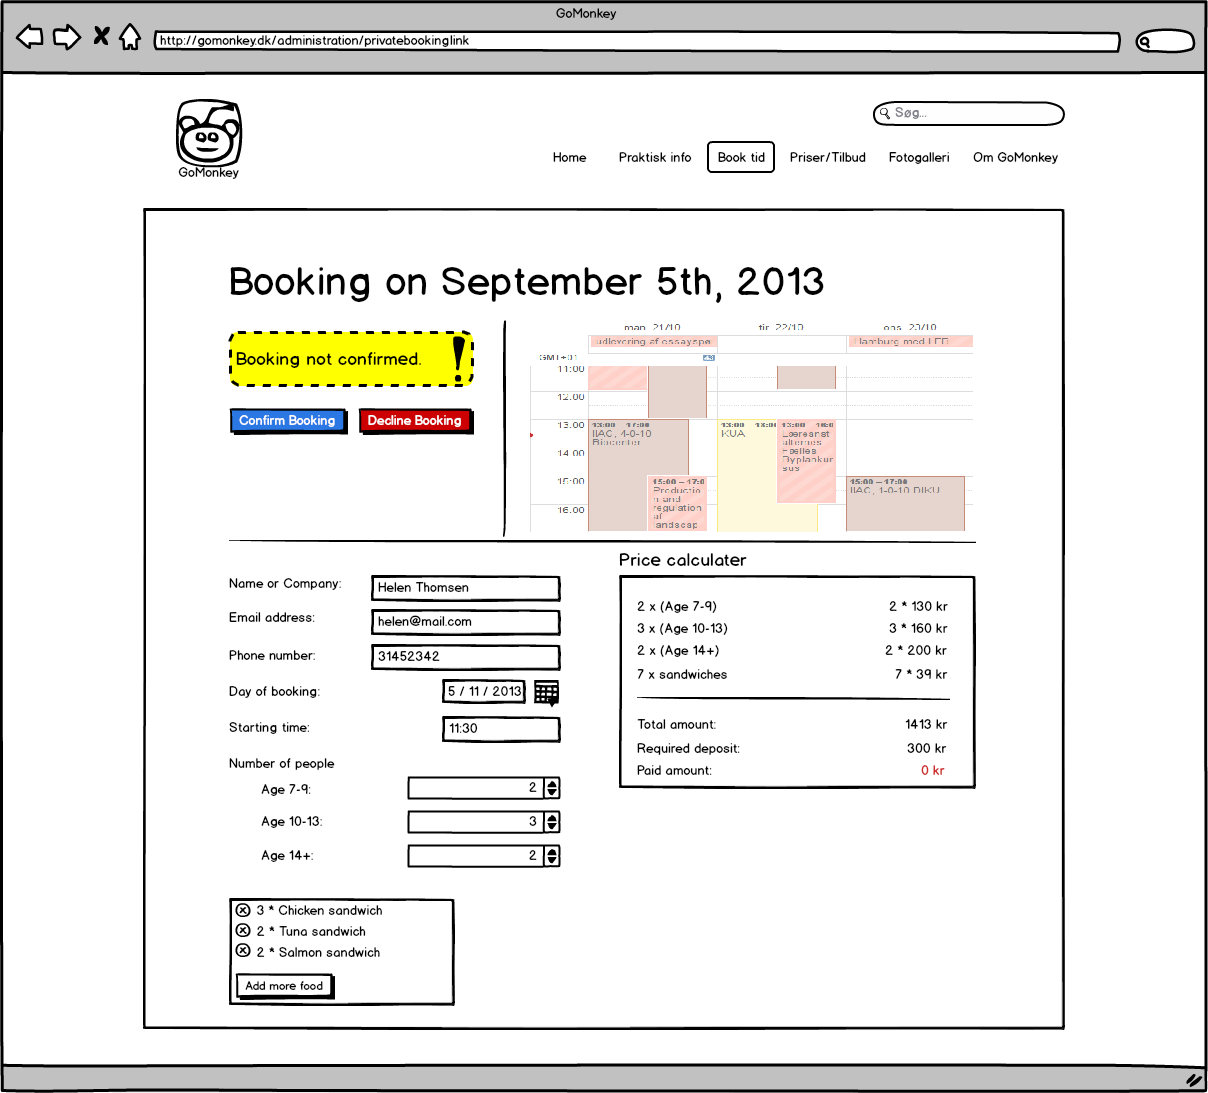
\includegraphics[width=.6\textwidth]{figures/mockup/admin_booking.png}
	    \caption{The manager can view the booking and see the calendar dates surrounding the booking.}
        \label{fig:admin}
\end{figure}

Confirming a booking causes an e-mail to be sent to the user notifying them of
this and also updates the user-viewable booking payment page to reflect that the
booking has been confirmed. A confirmed booking is eligible for payment, as per
the previous description of the customer booking payment page.

\begin{figure}[htbp]
    \centering
        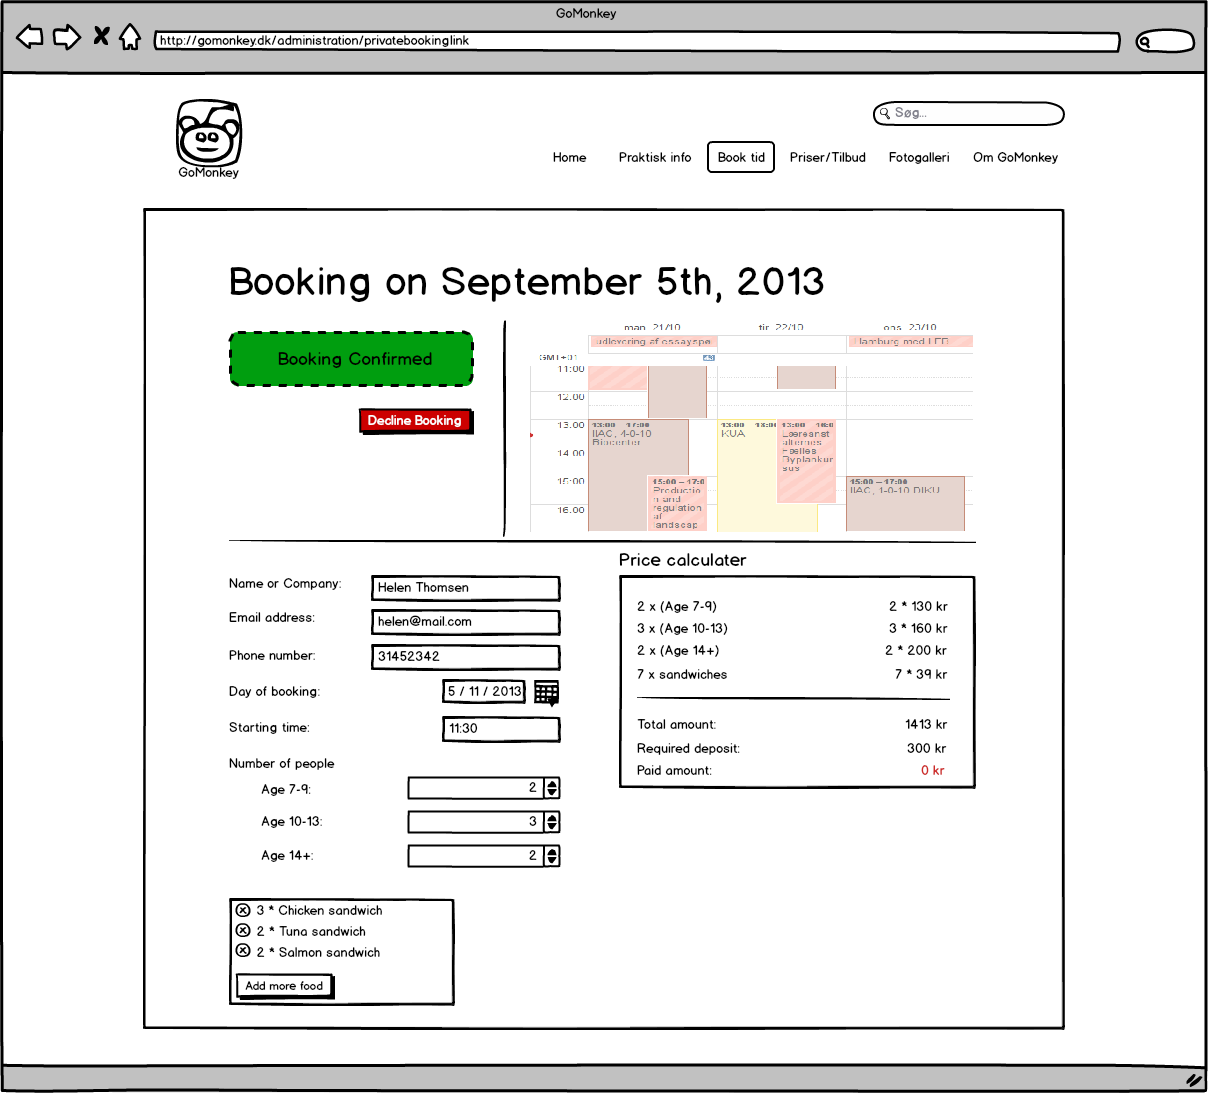
\includegraphics[width=.6\textwidth]{figures/mockup/admin_booking_confirmed.png}
	    \caption{The manager has confirmed and the customer can now pay for the session.}
        \label{fig:adminconfirmed}
\end{figure}

Declining a booking opens a modal popup that lets the administrator decide what
decline message to send the customer in an e-mail. The booking payment page
viewable by the customer will also reflect that the booking has been declined.
The decline booking popup can be seen in \autoref{fig:admindecline}.

\begin{figure}[htbp]
    \centering
        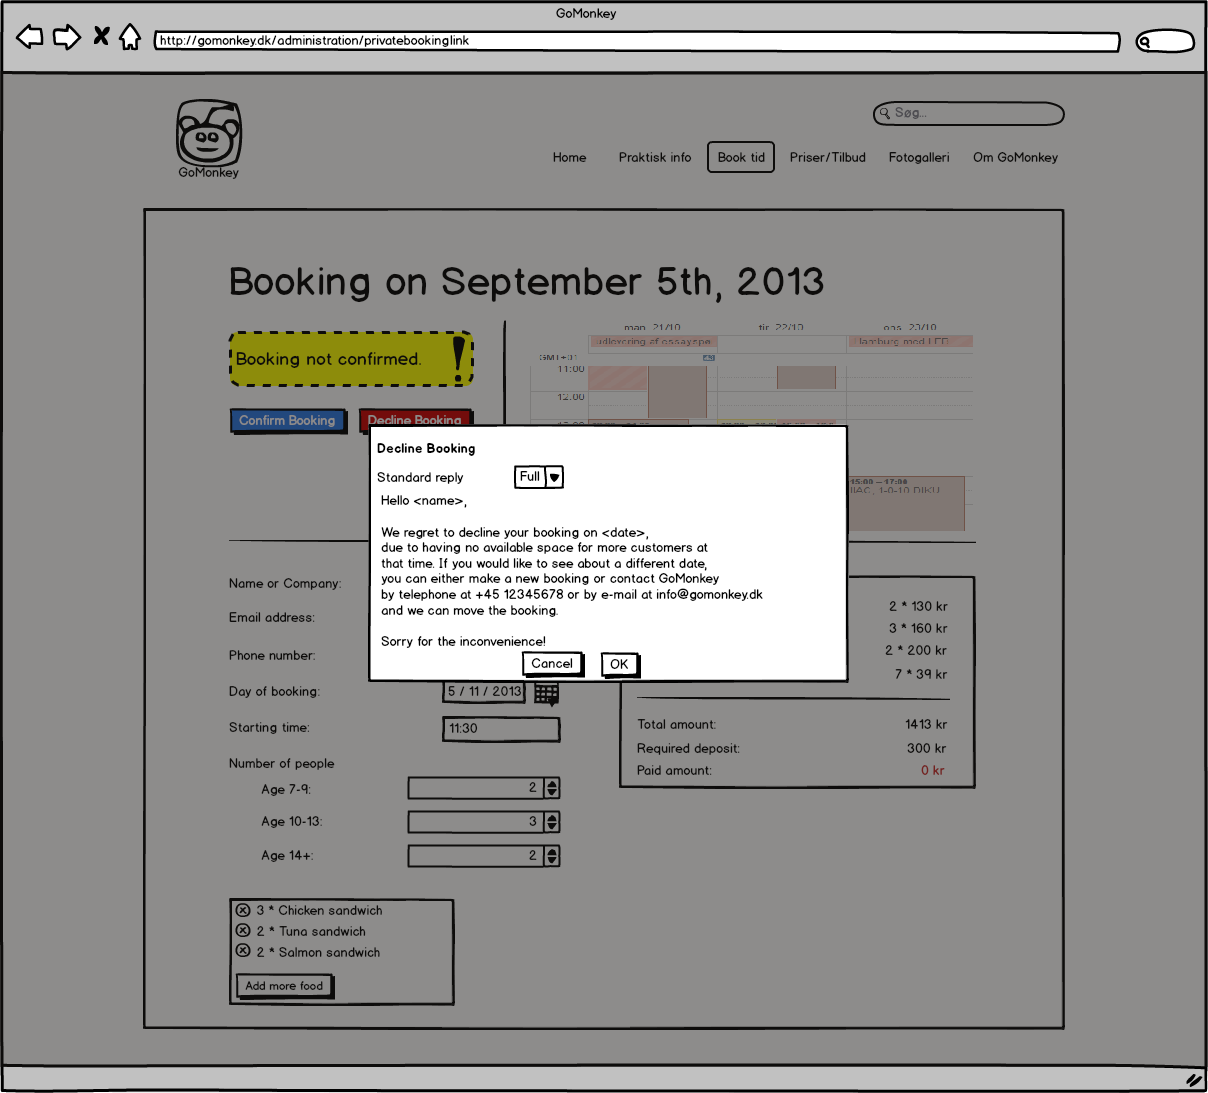
\includegraphics[width=.6\textwidth]{figures/mockup/admin_booking_decline.png}
	    \caption{The manager can decline the booking with a message describing why he had to decline, or attach a custom message.}
        \label{fig:admindecline}
\end{figure}

\FloatBarrier
\newpage

The last of the components is `An administrative overview of the current days
bookings', seen in \autoref{fig:overviewtoday}. This is intended for the
currently working employee to get a quick overview of the day. 

\begin{figure}[htbp]
    \centering
        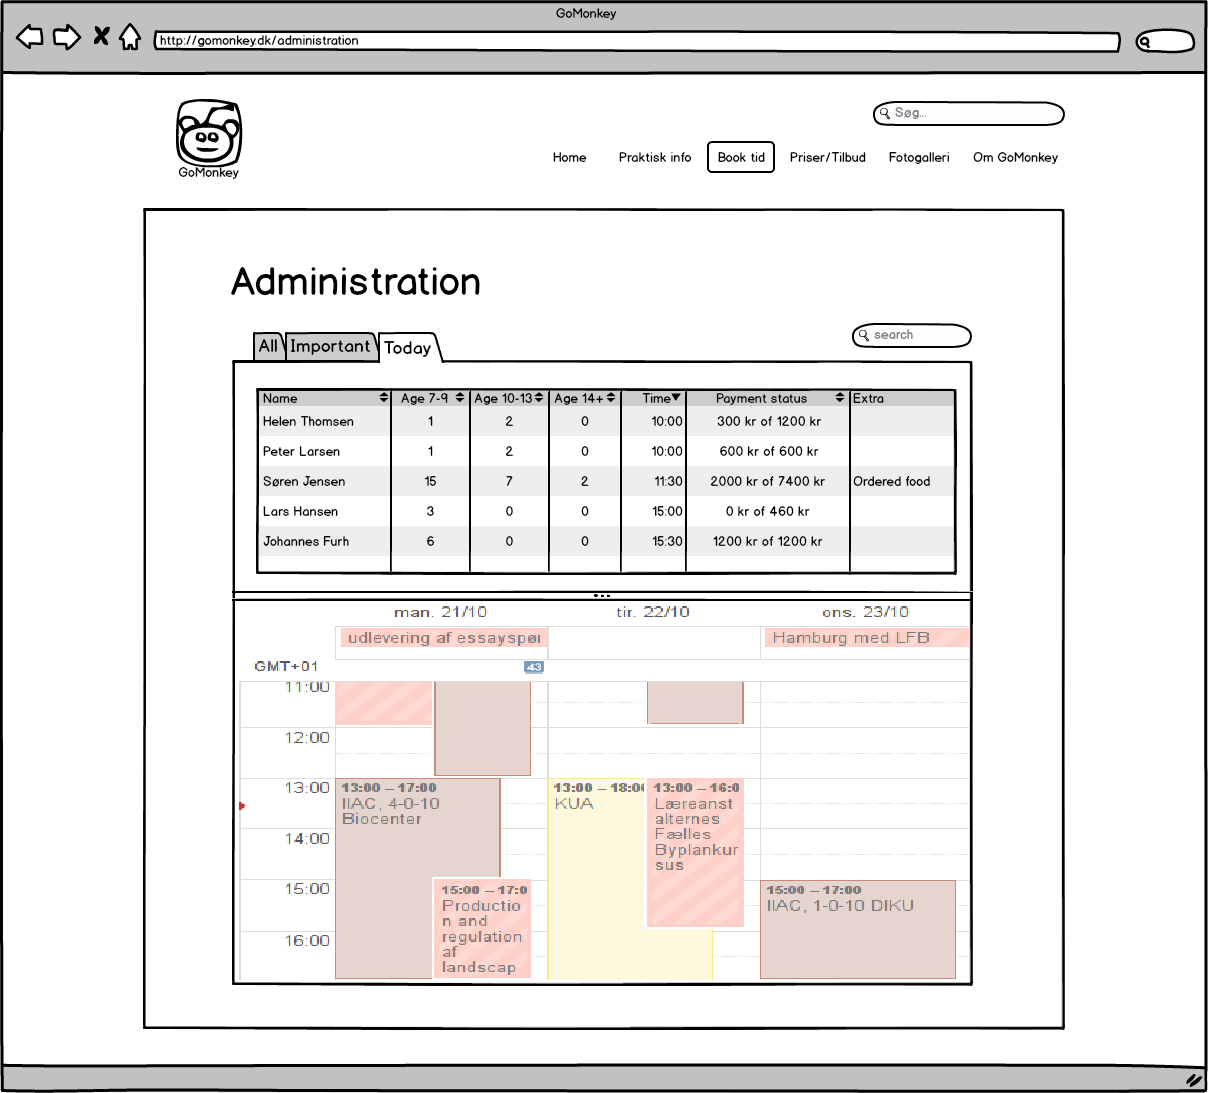
\includegraphics[width=.6\textwidth]{figures/mockup/overview_today.png}
	    \caption{The instructor can easily see what times there will be incoming groups.}
        \label{fig:overviewtoday}
\end{figure}

\newpage
\section{Finances and costs}
We suggest here an estimate of how much we believe the system will cost. This
is based on the design teams knowledge of pricing IT systems and their 
prior experiences with such projects. 

To build the system it is necessary to hire a programmer and a graphics artist.
It is also necessary to have a server running permanently, hosting the system. 
The prices of those are estimated to be:

\begin{itemize}
\item Front-end programmer, \textbf{500DKK/hour}
\item Graphics artist, \textbf{500DKK/hour}
\item Server hosting, \textbf{100DKK/month}
\end{itemize}

We estimate the following time requirements:

\begin{itemize}
	\item 30 hours of a programmer, to turn mockups into an initial prototype and integrate with the existing site.
	\item 10 hours of a graphics artist in total, to create art assets for the website.
\end{itemize}

This brings the total cost of such a venture to \textbf{20.000DKK} plus, for the 
development of the system. During the development phase, the server hosting
fees will also have to be paid, and is added over the course of development.

After the development period, the server hosting fee will still have to be paid
for as long as the system must remain online and usable. 

If annual maintenance of the booking system is required, such as security
updates and server maintenance, such a service is estimated to 10 hours per year
at a cost of \textbf{5.000DKK/year}.

\section{Changes to the work organization}
No fundamental changes occur to the structure of the organization as a whole.
The booking system may warrant a higher level of responsibility being taken by
instructors, but no additional workforce is required and no major restructuring
is considered to be necessary.

\section{Required qualifications}
It is assumed that administrative users of the system  be competent with a Personal Computer, 
use of web browsers and a light-weight administrative system. It is also assumed that the
user understands what the five components of the system are and
how they integrate with each other. In particular it is important to understand
how a booking occurs, and what the possible outcomes are: unpaid bookings vs.\ 
paid bookings, declined vs.\ confirmed bookings.

Customers require no qualifications above those of being able to use an Internet
browser, an e-mail client and a computer, in order to make a booking through the 
digital booking form.

\section{Advantages and disadvantages of implementation}
\subsection{For customers}
This section describes how the results of implementing the coherent vision will 
effect the user experience of customers in both positive and negative 
directions.

\begin{description}
\item[Advantages]
Previously, a lot of communication was very cumbersome, but 
with the new system, much of the communication is no longer needed. The 
ordering of food and exchange of necessary information is now handled by the 
new booking form, which will in turn be a more efficient work practice.

The reduced amount of cumbersome communication and easily understandable system
will also be partly visible for the customer, since the company will seem more
professional.

\item[Disadvantages]
The reduced amount of personal communication may lead the the booking process having
a less personal feeling for the customer. Knowing that you are writing with
another human being that actually caters for your specific needs is a very 
powerful effect, which will not be as utilized in the future system. 
\end{description}

\subsubsection{\gomonkey{} employees}
This section describes how the new system will help the staff do their 
job, and what drawbacks there may be, in relation to the old system.

\begin{description}
\item[Advantages]
The new system will be an
advantage for the instructor at work to have a more of the needed information
at hand, such as decifit price and amount and age of the coming customers. 
This will make for a less error prone handling of customers. The 
decifit price will be available to the instructor, instead of having to 
calculate the price manually. Further, the situation where a customer paid on 
the day and thus the instructor can't see the paid amount will completely be 
avoided, since the system is built to only support payment processors with 
instant transaction confirmations.

\item[Disadvantages]
The manager is very invested in the system, and will want the employees to 
use the system as soon as possible. The instructors may be less ready for the change and may
oppose spending time learning a new system. This can result in friction between
the two groups and can potentially result in a very uncomfortable work 
environment. 
\end{description}

\subsubsection{Business goals}
This section describes how the proposed system helps advance the company towards their 
business goals defined earlier in the report. 

\begin{description}
    \item[Become a self-sustainable climbing company with customers on a daily
        basis] The system does not advance this business goal directly.

    \item[Minimize time requirements pr.\ booking/customer] The system will
        support most of the situations which currently require a lot of
        correspondence between the manager and the customer. There is
        no need to check the bank account, which is a time consuming task, and
        very prone to errors. The requirement for intervention from the manager
        is drastically reduced in the new system, because many of the manual
        tasks are automated.

    \item[Minimize staff requirements to keep costs low] The system does not
        advance this business goal directly.

    \item[Increase sales (such as selling food and drinks)] A system that
        directly supports food sales is likely to generate a larger income off
        of this auxiliary service, than the existing booking form which has no
        such support.
\end{description}

\newpage
\section{Implementation strategy and plan}
The following section is a suggested step-by-step guide on how to develop, 
deploy and implement the new system into the current work organization. We 
will refer to a project manager, which may very well be the owner and 
manager of \gomonkey{}.

\subsection{Rent a server}
In order to host a service that can become part of the main website, a server
must be acquired which supports access to a database and webserver software. As
\gomonkey{} has no permanent or even temporary IT staff, purchasing a server to
place on-site is strongly discouraged. Instead, a cheap, minimally specced server 
should be provisioned from a hosting provider such as \url{www.hetzner.de}, 
\url{www.tdchosting.dk} or \url{www.rackspace.com} for a low monthly fee. This
removes the burden of maintenance and hardware failure from \gomonkey{}, which
is an important consideration for a small company.

\subsection{Hire a development team}
To facilitate the development of a custom system, a programmer and graphics
artist should be hired. In this report we assume that two individuals are found
and contracted individually, at the necessary stages of the project. Initially,
an IT consultant with technical skills within frontend development should be
found. Examples of relevant technologies are \textit{JavaScript, HTML, CSS, AJAX
and PHP}. The programmer should also have knowledge of RDBMS-based databases,
and preferably have prior experience implementing CRM-systems or similar.

Once the programmer has been contracted, relevant documentation for the system
should be passed on to the programmer, in order to inform them as best possible.
This report serves as the primary documentation of the system and its intent,
supported by the mockups and presented work flow.

Near the end of development, a graphics artist should be contracted to draw
relevant art for the pages, particularly those that customers can visit.
Estimates for costs and time required by this team have already been provided.

\subsection{Privately test the new system}
The system should be rolled out in testing privately first. At this point in
time, the employees and manager of \gomonkey{} can test the system and verify
that it satisfies all of the requirements. This can also serve as a good
opportunity to provide training to any employees that need to be able to also
handle booking, either through a workshop-format or paper-based instructions.

\subsection{Replace the old WordPress-based booking form}
Once the system is ready and the relevant employees are trained in using the
system, it can be released into the live environment and replace the existing
booking form and e-mail flow.

\newpage
\section{A standard system as an alternative}
A standard system can often lead to a cheap and easy solution to an immediate
problem.  We have compiled a list of three very possible candidates as a
supplier for a standard system.  After deep testing sessions of all systems, we
realized that none of them can solve the problems encountered at \gomonkey{}.
The testing session included creating a free temporary booking system. All
systems tend to have this feature, so potential customers can evaluate the
usefulness prior to paying. Attempts were then made to setup the system to
support the needs of \gomonkey{}, and after testing the usefulness of the
result, we could conclude upon the advantages and disadvantages of implementing
the system.

\begin{description}
\item[SuperSaaS] is a Joomla! plugin resembling a booking system, that integrates with a 
backend hosted at SuperSaas.

We decided not to use SuperSaaS, since the booking doesn’t support the required 
fields for the booking. A `form' can be attached to a booking after submitting 
initial information (intial information being the date and time of booking, 
name, phone number and email address), and this 
form can include extra information about amount of people in each age group, the
type of customer and food. This information can only be seen after two clicks 
from the calendar overview, thus making it impossible to get a good overview of 
how `available' a time slot is.

Furthermore, it is not possible to calculate a price based on the custom fields 
in the form, and as such, the system cannot ask for a deposit so we will still 
need another payment processor.

\item[onlinebooq.dk] promises a highly customizeable system which can be embedded into
any other existing system.

We did not manage to fit onlinebooq.dk with the requirements of \gomonkey{}.
They support selling 
`services', but unfortunately they only support selling one of each servive.
This can be seen in \autoref{fig:onlinebooq} as the checkbox, next to the 
service in question. This makes it useless for \gomonkey{}, since the price is 
calculated from the amount of people utilizing each service. It does support 
paypal and quickpay, but this doesn't matter if we cannot calculate the price 
correctly.

\begin{figure}[htbp]
    \centering
        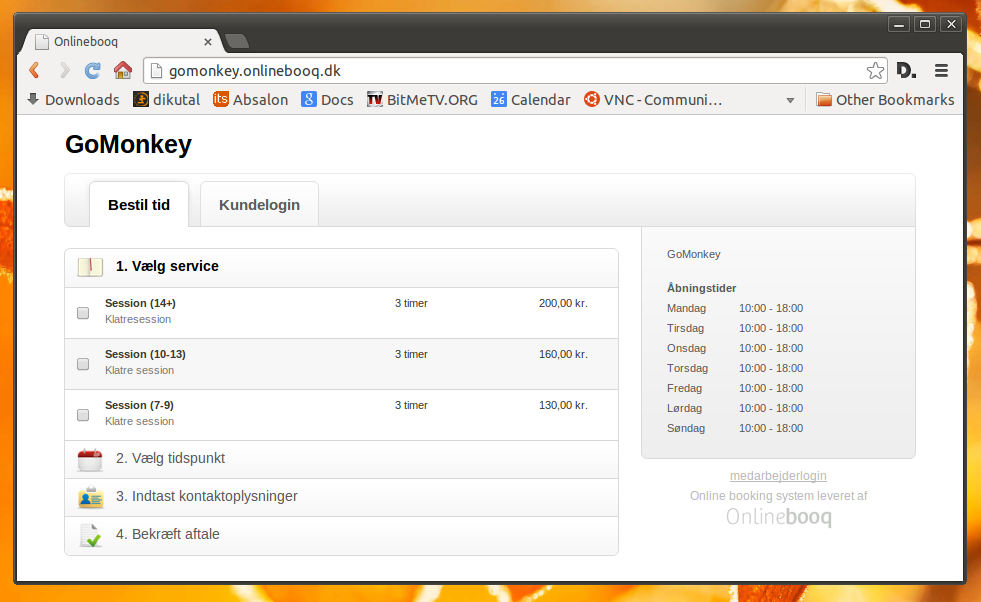
\includegraphics[width=1\textwidth]{figures/onlinebooq.png}
	    \caption{Screenshot from testing onlinebooq.dk.}
        \label{fig:onlinebooq}
\end{figure}
		

\item[Cyberbooking] brands itself as a cheap and simple alternative which runs great 
on mobile devices. 

It turned out to be impossible to fit the services of Cyberbooking with \gomonkey{}. 
Cyberbooking offer two types of 
calendars, one which supports one resource (e.g.\ a hairdresser) who can only
perform one service at a time. The other type supports booking slots on 
predefined events, (e.g.\ a fitness session) and the events are set by the 
company. None of these types can help \gomonkey{} with the booking process,
since the amount of resources aren't limited to one group of customers, and 
the times of bookings are very flexible.
\end{description}

While it is certainly possible to adjust the current work practices to use one of the
mentioned standard systems, this will result in huge changes to the current work
practices, which the design team judge to be very difficult to implement. When weighed
against the alternative of just keeping the current system, we concluded that time would 
be better spend on designing a custom system.


%\subsection{}
%To build a custom piece of software, it is suggested that \gomonkey{} contract
%both a programmer and a graphics artist, either as a package deal, from a
%software house or individually. Whichever choice is made, there are some
%important considerations for this aspect of the project.

%\begin{description}
%    \item [Leveraging the design project] This report should be seen as a guide
%        that can also be passed on to a programmer, in order to help the programmer
%        come to terms with the intended functionality of the system, the
%        reasoning behind the functionality and how such functionality could
%        look and act.
%    \item [
%\end{description}

%\subsection{Needed software and hardware}
%It is a requirement that the main website continues to run on the 
%WordPress which is hosted with One.com. This will make
%sure that the website maintains it's current, existing Google page-rank. Related 
%to this, the system will have to be embedable into WordPress. 

%It is necessary to have a server for hosting the new system, with 
%access to a database and a webserver. This is not achievable on the server from 
%One.com, so another will have to be purchased or rented. It will be sufficient to have 
%interfaces to a database and a webserver, but it is optimal to have root acess
%to the server.

%The server can run any operating system requested by either the developers or
%the manager, but picking a free system will avoid the costs of licenses for 
%proprietary systems.

%Additionally, there will still be parts of the original system which remain. 
%The scheduling and journaling of staff will still be hosted in the company's 
%Google Drive. 
%\subsection{Technical implementation}
%The project manager will have to contract an IT solutions supplier who 
%master the required knowledge of building the suggested system. They need
%a graphics artist and a programmer with knowledge of how to build a system
%which is embedable into a WordPress installation. The developing entity
%should read the design report prior to agreeing to the contract and
%price. 

%The projects responsible and the developers will have to agree on what server
%hosting supplier is chosen for the system, since \gomonkey{} will have to maintain
%contact with the supplier, even after the system has been developed. The 
%developers should also have an effect on what supplier is chosen, to ensure that
%they have the necessary access and tools to perform the development of the
%system. Possible suppliers could be either german Hetzner, danish
%Rackspace or Amazon.

%During the development phase, it should be possible for the project responsible
%to monitor the progression of the system, to ensure that misconceptions are 
%caught as early as possible.This will help keep the deliverables on track with
%the set time schedule. If this fails, a fair agreement on who pays for the 
%extra work should be worked out in the initial contract with the developers.

%Once the system has been developed by the developing entity, the manager should meet up with 
%them, and they should perform thorough manual testing and play scenarios, 
%attempting to visualize how the system will work with a customers. The
%developers have probably built even more webpages or some other way to view 
%log files and other monitoring tools, which should also be shown to the manager. 
%This will help the manager perform simple surveillence of the systems health.

%Finally, the developers should deliver a thorough documentation of the 
%delivered system which can be passed on to anyone who should be required to 
%perform maintenance or further development on the system. This will drastically
%reduce the price of such future interventions related to the IT system itself.

%\subsection{Specific qualifications required in using the new system}
%We assume that the instructors are familiar with using a calendar overview from 
%the current system. They will 
%still have to be shown how to navigate to the view of the bookings on the 
%current day, and how to interpret the information which is now visible.

%The manager and owner need deep knowledge of the system, and how bookings are to 
%be managed and handled. It will be necessary to introduce the system to a level
%where the manager and owner feels comfortable using the system, and teaching 
%the instructors how they should use the system.

%The booking form is tailored to help a customer perform the desired booking with 
%as few errors as possible. We assume that the customer uses the internet on a 
%weekly basis. The ease of using the booking formula was a 
%requirement for designing the booking form, so the necessary information and
%guidance is available to the customer to avoid any frustration that confusion
%could result in.

%\subsection{Advantages and disadvantages of the future system}
%In this section we will describe what advantages the vision will bring to 
%\gomonkey, in relation to the current situation. This will help weigh the
%benefits against potential costs and downsides.

%\subsubsection{Business goals}
%Here we describe how the proposed system helps advance the company towards their 
%business strategy, which was defined earlier in the design report. 

%\begin{description}
%\item[Become a self-sustainable climbing company with customers on a daily basis]
%To become self-sustainable company, it will be necessary to have enough profit
%to not have to sort to 'solving emergencies'. The owner will have to be able 
%to leave most of the work to employees, without taking a significan hit in 
%profit. This system puts the booking in a very defined process, and thus 
%simplifies it a lot. It becomes a lot simpler, so the manager will,
%with the correct employee, be able to pass on the task, to focus on other parts
%of the company.

%Economically, it is hard to define an absolute increase in profit, and the 
%result may only be achieved some time after deploymen. And, since 
%\gomonkey{} is such a new business, it is going to be very difficult to account
%the measured differences to the implementation of the system, since we know 
%nothing of the 'average' income.

%\item[Minimize time requirements pr.\ booking/customer]
%The system will support most
%of the situations which currently require a lot of correspondance between the 
%manager himself, and the customer. There is no need to check the bank account,
%which is a time consuming task, and very prone to errors. The requirement for 
%intervention from the manager is drastically reduced in the new system, because
%many of the manual tasks are automated.

%\item[Minimize staff requirements to keep costs low]
%The system does little to actually minimize staff, but indirectly, the manager
%can, with more time at hand, do more work to coordinate staff in a more 
%economically viable manner. Further, when the company gets more customers,
%there will be less situations where it is necessary to staff a situation where
%there is only a low income, which has occurred and often resulted in a declination
%of the booking.

%\item[Increase sales (such as selling food and drinks)]
%The system supports selling more than just the single service of a visit to a climbing park. It is a lot
%easier for customers to buy additional services, such as food and drinks, due to 
%the direct support for this in the new system, compared to the complicated 
%process of offering, accepting and ordering food.
%\end{description}

%\subsubsection{Groups of staff and their relations}
%This section describes how the new system will help the staff do their 
%job, and what drawbacks there may be, in relation to the old system.
%
%\begin{description}
%\item[Advantages]
%The new system will be an
%advantage for the instructor at work to have a more of the needed information
%at hand, such as decifit price and amount and age of the coming customers. 
%This will make for a less error prone handling of customers. The 
%decifit price will be available to the instructor, instead of having to 
%calculate the price manually. Further, the situation where a customer paid on 
%the day and thus the instructor can't see the paid amount will completely be 
%avoided, since the system is built to only support payment processors with 
%instant transaction confirmations.

%\item[Disadvantages]
%The manager is very invested in the system, and will want the employees to 
%use the system as soon as possible. The instructors may be less ready for the change and may
%oppose spending time learning a new system. This can result in friction between
%the two groups and can potentially result in a very uncomfortable work 
%environment. 
%\end{description}

%\subsubsection{Customers}
%This section describes how the results of implementing the coherent vision will 
%effect the user experience of customers in both positive and negative 
%directions.

%\begin{description}
%\item[Advantages]
%Previously, a lot of communication was very cumbersome, but 
%with the new system, much of the communication is no longer needed. The 
%ordering of food and exchange of necessary information is now handled by the 
%new booking form, which will in turn be a more efficient work practice.

%The reduced amount of cumbersome communication and easily understandable system
%will also be partly visible for the customer, since the company will seem more
%professional.

%\item[Disadvantages]
%The reduced amount of personal communication may lead the the booking process having
%a less personal feeling for the customer. Knowing that you are writing with
%another human being that actually caters for your specific needs is a very 
%powerful effect, which will not be as utilized in the future system. 
%\end{description}

%\subsection{Organizational implementation}
%A new IT system will affect the whole 
%organization, and thus it is necessary to prepare for the changes, and be very
%vigilant when adapting the company to a new system. 

%The requirement for organizational preparation arises after the system has been
%put into production. It is necessary for the employees to be prepared for
%switching to a new system. This can be done by informing the employees about how the project is coming along, over 
%the course of the development. This will give the employees a chance to accept 
%the changes over a longer period, 
%giving the idea time to 'sprout and bloom' before they will need to use the 
%system. This will increase the readiness for change.

%When the system is finished, and ready to be used, the manager should perform
%a training session with the employees. This can be done with every single
%instructor, or by inviting all of them for a single session, depending on what
%the manager feels most comfortable with. The session should include showing most of 
%the system, even the parts they will not use themself. Performing scenarios
%with the instructors, using the new system will further help the understanding
%of their new role. This session will give the instructors the final idea
%of why the system is good for the company, and equips them for guiding the 
%customers in a better way, since they are aware of the whole user experience.

